% seqhesion whitepaper -- FIRST DRAFT for review.
% Build: latexmk -pdf seqhesion.tex   (see README.md)
\documentclass[11pt,a4paper]{article}

\usepackage[T1]{fontenc}
\usepackage[utf8]{inputenc}
\usepackage{lmodern}
\usepackage[margin=2.2cm]{geometry}
\usepackage{microtype}
\usepackage{amsmath,amssymb}
\usepackage{booktabs}
\usepackage{tabularx}
\usepackage{xcolor}
\usepackage{tikz}
\usetikzlibrary{positioning,arrows.meta,fit,backgrounds}
\usepackage[font=small,labelfont=bf]{caption}
\usepackage{enumitem}
\setlist{nosep,leftmargin=*}
\usepackage[round,authoryear]{natbib}
\usepackage[colorlinks=true,linkcolor=blue!50!black,citecolor=blue!50!black,urlcolor=blue!50!black]{hyperref}

% Visible placeholders for numbers and details still to be filled in.
\newcommand{\todo}[1]{\textcolor{red}{\textbf{[TODO: #1]}}}

\newcommand{\seqhesion}{\textsf{seqhesion}}
\newcommand{\level}{\ell}

\title{\seqhesion: a label-blind hierarchy of fungal ITS sequences\\
from many small overlapping trees\\[0.5ex]
\large Draft}
\author{Josh Walker\\ \small Independent Researcher \and Claude Code\\ \small (Claude Opus 5.5, Anthropic)}
\date{Draft of 6 October 2026}

\begin{document}
\maketitle

\begin{abstract}
Community DNA-barcoding programmes now sequence the nuclear ribosomal internal transcribed spacer
(ITS) of tens of thousands of vouchered fungal collections, often far faster than taxonomists can
name them. Many of these sequences carry provisional, inconsistent or missing names, so any grouping
that leans on the names inherits their errors. \seqhesion{} (``sequence cohesion'') groups sequences
from sequence evidence alone. It builds thousands of small phylogenetic trees (\emph{shards}) over
overlapping neighbourhoods of about 150 sequences each. For every pair of sequences, each shard that
holds both records the diameter of the smallest clade containing them; the median over shards is
the pair's join level. Average linkage over the observed pairs only gives a hierarchy cut at fixed
tree-distance levels. Every group carries its evidence: cohesion, pull towards outside groups, and
their difference, the \emph{margin}, which predicted which groups recur when the shard trees are
resampled (AUC 0.94). Coarser structure comes from separate layers of stratified sparse shards,
first within each connected component and then across components. Group identities
(\emph{antenomina}) persist across releases by a mutual-best-match rule, and partial ITS2-only
sequences are placed onto the stored shard alignments without changing the hierarchy. On a corpus
of 225,876 input sequences, drawn mainly from MycoMap with other sources (146,875 distinct full-ITS sequences in 4,172 components),
\seqhesion{} produced 50,847 fine-level groups with per-group confidence. It is an evidence layer
and a navigation aid for curators, not a phylogeny. This paper describes the method, the choices
behind it and their limits, and the in-house experiments that support them.
\end{abstract}

% =====================================================================================
\section{Introduction}

The ITS region is the formal DNA barcode for Fungi \citep{schoch2012its}, and community science has
made it cheap to sequence. Programmes such as MycoMap sequence vouchered macrofungal collections
made by volunteers, increasingly with nanopore long reads, and publish the consensus sequences
with whatever name the collector or an identification tool assigned. The result is a large,
fast-growing corpus in which much of the diversity is undescribed or only provisionally named, many
names are field identifications, and the same taxon may appear under several names, or several taxa
under one.

Two common ways of organising such a corpus both depend on names or fixed identity thresholds.
Reference-based identification assigns each sequence the name of its closest match. Threshold
clustering, such as the species hypotheses of UNITE \citep{koljalg2013unite,abarenkov2024unite},
groups sequences by single-linkage identity at a few fixed distances. Studies of ITS variation
show that no single identity threshold separates species across the fungal kingdom
\citep{nilsson2008its,vu2019its}. Even within one genus such as \emph{Cortinarius}, the best
threshold varies by lineage \citep{garnica2016cortinarius}.

\seqhesion{} takes a different position. It is an \emph{evidence layer}: it groups sequences
purely from the sequence data and reports, for every group, how strongly the data support it.
Names never enter any decision. Labels may travel with the input for display, but nothing in the
processing path reads them. Choosing which groups become named units is curation, and happens
downstream in a separate tool that maps names onto \seqhesion's groups. Agreement with names is
used only as a sanity check, never as a target to optimise. We call the design \emph{label-blind}.

Being label-blind has three practical consequences.
\begin{enumerate}
  \item The groups cannot inherit misidentifications. A curator who finds a name scattered over
        several well-supported groups learns something about the name.
  \item The output does not depend on the state of the taxonomy. Undescribed lineages are first-class
        groups with their own persistent identifiers (\emph{antenomina}, ``before the name'',
        Section~\ref{sec:antenomina}), to which comments and curation can attach before any name exists.
  \item Validation must use something other than names. We use reproducibility under independent
        resampling of the shards, and treat name agreement only as a display.
\end{enumerate}

The second idea is to build from many small trees rather than one large one. A single alignment of
tens of thousands of ITS sequences is not credible: ITS is alignable only among fairly close
relatives. A single tree, even if feasible, gives one topology with no indication of which parts
would survive a rebuild. \seqhesion{} instead builds thousands of small trees over overlapping
neighbourhoods, each from a carefully aligned set of about 150 related sequences. It then pools
what the trees say about every pair of sequences. The overlap is the source of the confidence
measures. Pairs that no shard holds are treated as missing evidence, not as evidence of distance.

This paper is a first description of the method and its current results. Section~\ref{sec:related}
places it in the literature. Section~\ref{sec:method} describes the pipeline, and
Section~\ref{sec:impl} its implementation and reproducibility guarantees.
Section~\ref{sec:results} reports in-house experiments, and Section~\ref{sec:limits} states the
limitations plainly.

% =====================================================================================
\section{Related work}\label{sec:related}

\paragraph{ITS barcoding and reference clustering.}
The ITS region was proposed as the primary fungal barcode for its high rate of successful
identification across the kingdom \citep{schoch2012its}, building on the DNA barcoding programme
of \citet{hebert2003barcoding}. UNITE organises ITS sequences into species hypotheses (SHs) by
clustering at a series of distance thresholds within higher-level groups, with experts choosing
the threshold for each lineage \citep{koljalg2013unite,abarenkov2024unite}. The Barcode Index
Number system of BOLD gives animal COI clusters persistent registry identifiers
\citep{ratnasingham2013bin}. Our antenomina serve a similar purpose for tree-based groups.
Studies of intraspecific ITS variability show that fixed identity thresholds misclassify many
species \citep{nilsson2008its,vu2019its,garnica2016cortinarius}. Divergent intragenomic ITS copies
are common \citep{bradshaw2023intragenomic}, and apparent barcode gaps shrink as sampling becomes
more complete \citep{meyer2005barcodegap}. \seqhesion{} uses identity only to decide which sequences
are sampled together, never to group them, and reports structure at several levels instead of
choosing one threshold.

\paragraph{Single-locus species delimitation.}
Distance-based methods such as ABGD \citep{puillandre2012abgd} and ASAP \citep{puillandre2021asap}
find gaps in pairwise distance distributions. ASAP returns a ranked list of partitions from one
hierarchical clustering, the closest analogue to our multi-level output. Tree-based methods (GMYC
\citep{pons2006gmyc,fujisawa2013gmyc}, PTP and bPTP \citep{zhang2013ptp}, mPTP \citep{kapli2017mptp})
fit models of speciation and coalescence to a single tree. They need one tree over all sequences,
and some need it binary or ultrametric. They return a single partition, possibly with per-node
support. \seqhesion{} does not attempt species delimitation. It reports a nested set of groups, each
with its evidence, and leaves the choice of level, clade by clade, to curators.

\paragraph{Divide-and-conquer phylogenetics and supertrees.}
Large-scale alignment and tree estimation are commonly divided into subproblems: DACTAL
\citep{nelesen2012dactal} and PASTA \citep{mirarab2015pasta} work on overlapping or disjoint subsets
and merge them. uDance \citep{balaban2024udance}, used for Greengenes2
\citep{mcdonald2024greengenes2}, grows trees by placement and refines them per partition.
Supertree methods combine trees on overlapping taxon sets. These include Min-Cut
\citep{semple2000mincut}, the modified Min-Cut of \citet{page2002mincut}, which treats a polytomy
as missing information rather than conflict, the Greedy Strict Consensus Merger
\citep{fleischauer2016gscm} and the Spectral Cluster Supertree \citep{mcarthur2024scs}. The last
links taxa only when some input tree holds both, so a pair never seen together is no evidence.
\seqhesion{} shares that principle. It differs from these methods in its goal: it does not try to
produce a single resolved tree, only a hierarchy of groups with their evidence. It also never merges
trees: it pools what each tree says about pairs.

\paragraph{Consensus clustering.}
The co-association matrix of evidence-accumulation clustering \citep{fred2005evidence} records, for
each pair of objects, how often many base clusterings put them together. Hierarchical clustering of
that matrix then gives the final structure. Cluster ensembles \citep{strehl2002ensembles} include the
case where each base clusterer sees only a subset of the objects. Consensus clustering
\citep{monti2003consensus} normalises co-assignment by co-sampling: a pair's score is the number of
resamples that put it together divided by the number that contain both. It also defines per-item
and per-cluster consensus scores. Minipatch consensus clustering \citep{gan2022impacc} extends this
to tiny subsamples and adaptive sampling. \seqhesion's co-association is of this kind. Its base
``clusterings'' are shard trees, which hold neighbourhoods rather than random subsets. Each tree
contributes a continuous join level per pair rather than a binary co-assignment, and pairs no shard
holds are excluded from the linkage, not imputed.

\paragraph{Support and resampling.}
Felsenstein's bootstrap \citep{felsenstein1985bootstrap}, an application of
\citet{efron1979bootstrap}, measures the stability of splits under resampling of alignment
columns. The transfer bootstrap \citep{lemoine2018tbe} relaxes it for large trees. Taxon jackknifing
\citep{lanyon1985jackknife} perturbs the taxon set instead. \seqhesion's overlapping shards are
closer to a taxon jackknife combined with a re-run of alignment and inference. We validate the
confidence measures by bootstrap resampling of whole shard trees (Section~\ref{sec:res-confidence}).

\paragraph{Phylogenetic placement.}
Placement tools such as pplacer \citep{matsen2010pplacer} and EPA-ng \citep{barbera2019epang} attach
query sequences to a fixed reference tree without changing it. \seqhesion{} places partial
(ITS2-only) sequences in the same spirit. It adds them to stored shard alignments with MAFFT
\citep{katoh2012add} and re-infers the shard tree, reading the query's position from the
re-inference while the stored trees, and so the hierarchy, stay unchanged
(Section~\ref{sec:placement}).

% =====================================================================================
\section{Method}\label{sec:method}

\begin{figure}[t]
\centering
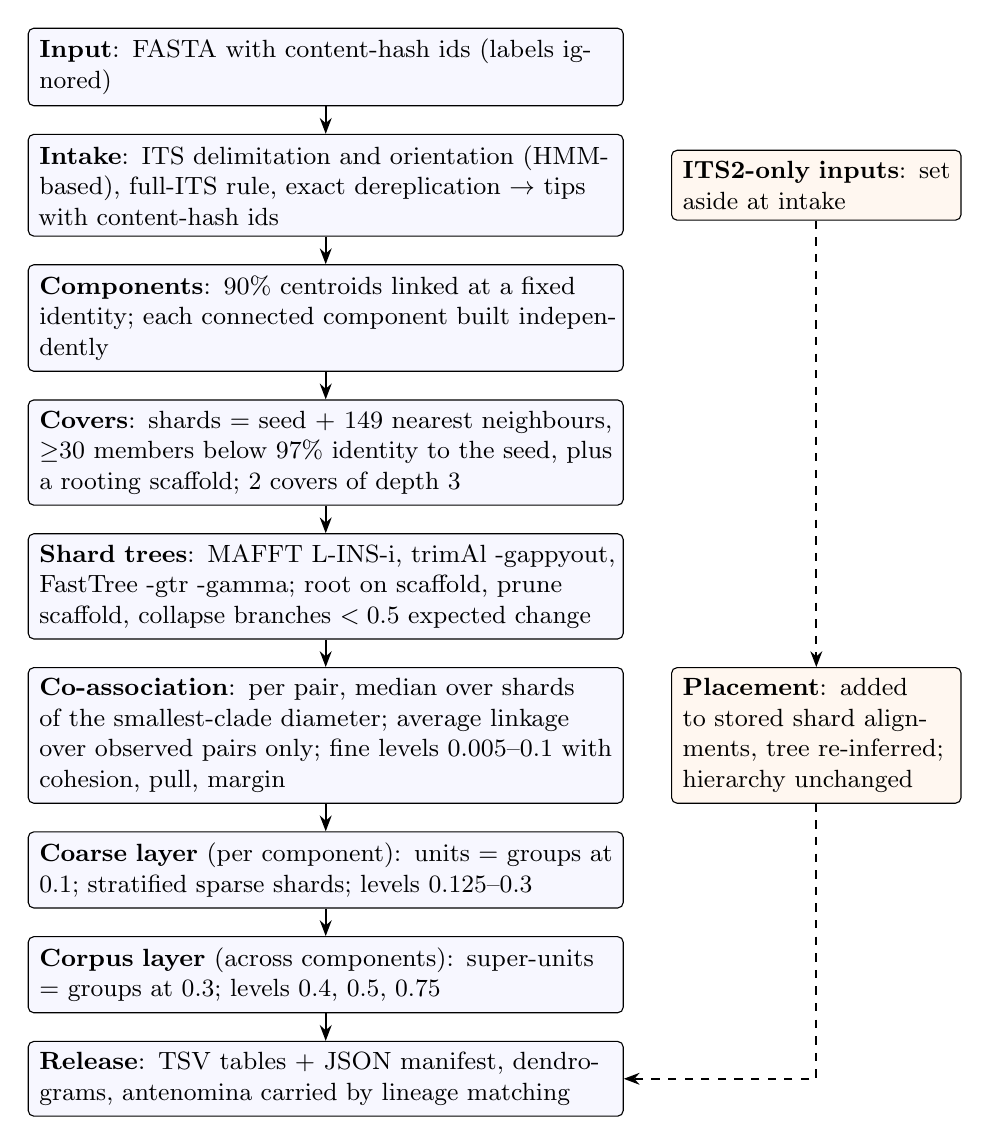
\begin{tikzpicture}[
  node distance=3.5mm,
  box/.style={draw, rounded corners=2pt, align=left, font=\small, text width=0.60\linewidth,
              inner sep=4pt, fill=blue!3},
  side/.style={draw, rounded corners=2pt, align=left, font=\small, text width=0.28\linewidth,
               inner sep=4pt, fill=orange!6},
  arr/.style={-{Stealth[length=2mm]}, thick}]
  \node[box] (in)   {\textbf{Input}: FASTA with content-hash ids (labels ignored)};
  \node[box, below=of in] (intake) {\textbf{Intake}: ITS delimitation and orientation (HMM-based),
      full-ITS rule, exact dereplication $\rightarrow$ tips with content-hash ids};
  \node[box, below=of intake] (comp) {\textbf{Components}: 90\% centroids linked at a fixed
      identity; each connected component built independently};
  \node[box, below=of comp] (cover) {\textbf{Covers}: shards = seed + 149 nearest neighbours,
      $\ge$30 members below 97\% identity to the seed, plus a rooting scaffold; 2 covers of depth 3};
  \node[box, below=of cover] (trees) {\textbf{Shard trees}: MAFFT L-INS-i, trimAl -gappyout,
      FastTree -gtr -gamma; root on scaffold, prune scaffold, collapse branches $<0.5$ expected change};
  \node[box, below=of trees] (coassoc) {\textbf{Co-association}: per pair, median over shards of
      the smallest-clade diameter; average linkage over observed pairs only;
      fine levels 0.005--0.1 with cohesion, pull, margin};
  \node[box, below=of coassoc] (coarse) {\textbf{Coarse layer} (per component): units = groups at 0.1;
      stratified sparse shards; levels 0.125--0.3};
  \node[box, below=of coarse] (corpus) {\textbf{Corpus layer} (across components): super-units =
      groups at 0.3; levels 0.4, 0.5, 0.75};
  \node[box, below=of corpus] (rel) {\textbf{Release}: TSV tables + JSON manifest, dendrograms,
      antenomina carried by lineage matching};
  \node[side, right=6mm of intake] (its2) {\textbf{ITS2-only inputs}: set aside at intake};
  \node[side, right=6mm of coassoc] (place) {\textbf{Placement}: added to stored shard
      alignments, tree re-inferred; hierarchy unchanged};
  \foreach \a/\b in {in/intake, intake/comp, comp/cover, cover/trees, trees/coassoc,
                     coassoc/coarse, coarse/corpus, corpus/rel}
    \draw[arr] (\a) -- (\b);
  \draw[arr, dashed] (its2) -- (place);
  \draw[arr, dashed] (place.south) |- (rel.east);
\end{tikzpicture}
\caption{The \seqhesion{} pipeline. Sequence identity (vsearch) is used only to decide what is
sampled together: components, shard neighbourhoods, the scaffold and candidate shards for
placement. Every grouping decision is made from tree distances in the shard trees.}
\label{fig:pipeline}
\end{figure}

Figure~\ref{fig:pipeline} summarises the pipeline. Table~\ref{tab:params} lists its main
parameters. Two rules run through all of it:
\begin{itemize}
  \item \textbf{Label-blind.} No step reads a name.
  \item \textbf{Tree distance and identity distance are not comparable.} Alignment identity
        (vsearch global identity) is used only to choose which sequences are sampled together.
        Every grouping and placement decision comes from tree distances: model-corrected, on
        trimmed alignment columns, with sub-resolution branches collapsed.
\end{itemize}

\begin{table}[t]
\centering\small
\caption{Main parameters of the current release.}
\label{tab:params}
\begin{tabularx}{\linewidth}{@{}lX@{}}
\toprule
Step & Setting \\
\midrule
Intake & full ITS: ITS1 $\ge$ 50, 5.8S $\ge$ 140, ITS2 $\ge$ 50 bp; an unanchored flanking spacer
         $\ge$ 150 bp; extracted full ITS $\le$ 3{,}000 bp \\
Components & vsearch 90\% centroids, linked at 86\% centroid identity (production setting) \\
Neighbourhoods & vsearch global search, identity floor 80\% (60\% for small components, corpus-wide) \\
Shards & 150 sequences (seed + 149 nearest); top-up to $\ge$ 30 members below 97\% identity to the
         seed; scaffold = 30 most abundant 85\% centroids \\
Covers & 2 independent covers, each sequence in $\ge$ 3 shards per cover \\
Trees & \texttt{mafft --localpair --maxiterate 1000 --thread 1}; \texttt{trimal -gappyout};
        \texttt{FastTree -gtr -gamma -nt} \\
Tree preparation & root on the scaffold tip farthest from the members; prune scaffold; collapse
        internal branches $< 0.5/W$ ($W$ = trimmed alignment width) \\
Fine levels & 0.005, 0.01, 0.015, 0.02, 0.03, 0.05, 0.075, 0.1 (substitutions/site, clade diameter) \\
Coarse layer & units at 0.1; 150 units per sparse shard; $\approx$24 expected shards per unit pair;
        8 outgroup sequences; levels 0.125, 0.15, 0.2, 0.25, 0.3 \\
Corpus layer & super-units at 0.3; 3 representatives per unit, neighbour identity floor 50\%;
        150 units per shard + 20 context units; 2 covers of depth 6; levels 0.4, 0.5, 0.75 \\
Antenomina & mutual best match by Jaccard over shared inputs, $J > 1/2$ \\
\bottomrule
\end{tabularx}
\end{table}

\subsection{Intake}\label{sec:intake}

Input sequences are identified by content hashes. An input's id is the smaller of the SHA-256
digests of the cleaned sequence and of its IUPAC-aware reverse complement, so the id does not
depend on orientation. \seqhesion{} recomputes every id and refuses the whole input on any mismatch
or duplicate. Anything after the id on a FASTA header is ignored.

The ITS subregions are delimited and the sequence oriented with pyitsx \citep{walker2026pyitsx}, an
HMM-based ITS extractor in the manner of ITSx \citep{bengtsson2013itsx}. A sequence counts as \emph{full ITS} when ITS1,
5.8S and ITS2 are all long enough (Table~\ref{tab:params}) and each flanking ribosomal anchor is
either present or, when missing, the spacer beside it is long enough that it was probably trimmed
at the boundary rather than truncated. Sequences with an LSU anchor and a usable ITS2 but an
incomplete ITS1 or 5.8S are classed \emph{ITS2-only}. They do not shape the hierarchy and are placed
on it afterwards (Section~\ref{sec:placement}). Chimeric, unreadable, overlong (over 3{,}000 bp;
real full ITS tops out near 2{,}500 bp) and otherwise incomplete sequences are dropped and counted
by class. Full-ITS extracts are exactly dereplicated. Each distinct extract is a \emph{tip}, with an
id derived from a hash of its sequence. Nothing is corrected: homopolymer errors, ambiguity codes
and intragenomic variants are kept and their effects reported downstream.

\subsection{Components}\label{sec:components}

The dereplicated tips are clustered into 90\% centroids (vsearch \texttt{--cluster\_fast}
\citep{rognes2016vsearch}), and centroids are linked when they match at or above a fixed identity
(86\% in the production build). Each connected component of this centroid graph is built
independently. The centroids only locate components. They never define groups.

Many components are small. In the production corpus, 44\% of tips lie in components of fewer than
150 tips, the size of one shard. Built alone, such a component could only be rooted on one of its
own tips. Instead, its tips draw their nearest neighbours from the whole corpus (identity floor
60\%), and these outside sequences serve only as rooting context. They are present in the tree,
pruned before co-association, and never grouped. A lab test found that 0\% of small-component tips
joined another component's tips at levels up to 0.075, so the pruning loses no grouping evidence.
Singletons and components with no usable neighbour get no tree.

\subsection{Shards and covers}\label{sec:covers}

A \emph{shard} is a seed tip plus its 149 nearest neighbours by vsearch global identity. A
\emph{cover} is a set of shards in which every tip lies in at least \emph{depth} shards (depth 3).
Seeds are chosen greedily from the least-covered tips, and a random stream only breaks ties, so
different streams give different but equally valid covers. No seed or member set is used twice
within a cover. Tips with too few neighbours to seed a full shard receive smaller shards made of
whatever neighbours they have, and every tip is accounted for as covered, under-covered or isolated.

Two refinements matter in practice.
\begin{itemize}
  \item \textbf{Context quota.} In a dense species complex the 149 nearest neighbours may all be
        near-identical to the seed, so the shard never shows the species against outsiders. Each
        shard is therefore topped up so that at least 30 of its members are below 97\% identity to
        the seed. Identity here decides only what is \emph{sampled}.
  \item \textbf{Scaffold.} Every shard also contains a fixed scaffold: the 30 most abundant 85\%
        centroids of the component. The scaffold provides rooting candidates and is pruned before
        any co-association is counted, since it sits in every shard and would otherwise link
        everything.
\end{itemize}

Two covers are drawn independently. In dense neighbourhoods they often draw exactly the same
member set; across the large components 55--61\% of cover-1 shards were such \emph{twins} of a
cover-0 shard. A twin is the same sample and gives the same tree, so it is built once and counted
once.

\subsection{Shard trees}\label{sec:trees}

Each shard is aligned with MAFFT L-INS-i \citep{katoh2005mafft5,katoh2013mafft}, run
single-threaded for determinism. The alignment is trimmed with trimAl \texttt{-gappyout}
\citep{capella2009trimal}, and a tree is inferred with FastTree under GTR with gamma-distributed
rates \citep{price2010fasttree}. Each tree is then prepared as follows.
\begin{enumerate}
  \item It is rooted on the scaffold tip farthest from the members (by mean patristic distance to
        the first 40 members).
  \item The scaffold is pruned.
  \item Internal branches shorter than $0.5/W$ substitutions per site are collapsed into
        polytomies. Here $W$ is the trimmed alignment width, so the threshold is about half an
        expected change. Branches this short carry no resolvable signal, and FastTree resolves
        them arbitrarily.
\end{enumerate}

\subsection{Co-association and the fine hierarchy}\label{sec:coassoc}

Let $S$ be the set of distinct prepared shard trees of a component, pooled over both covers with
twins counted once. For a shard $s$ holding tips $i$ and $j$, let $c_s(i,j)$ be the smallest clade
of $s$ containing both, and define the shard's \emph{join level}
\begin{equation}
  d_s(i,j) = \operatorname{diam}\bigl(c_s(i,j)\bigr) = \max_{a,b \in c_s(i,j)} p_s(a,b),
\end{equation}
where $p_s$ is the patristic distance in $s$. The diameter scale makes a level a statement about
the widest pair inside a group, not about its height above a root.

\paragraph{The ``identical'' join.}
At a polytomy, plain diameters put every pair of the polytomy's children at the polytomy's full
width. This split near-identical tips between groups. Following the view that a polytomy is missing
information rather than conflict \citep{page2002mincut}, two tips in different children of a
polytomy join at the diameter of just those two children, \emph{but only if} that span is at most
one expected change ($1/W$), i.e.\ when the data cannot tell them apart. Every other pair in the
polytomy joins at its full width. A variant that applied the narrower span to all polytomy pairs
grouped distinguishable lineages by noise-level distances, and in simulation it doubled the share
of wrong groups at level 0.03 (4.4\% to 8.6\%).

\paragraph{Pooling.}
A pair $(i,j)$ is \emph{observed} if at least one shard holds both. Its consensus join level is the
median over the shards that hold it:
\begin{equation}
  D(i,j) = \operatorname{median}\{\, d_s(i,j) : s \in S,\ i,j \in s \,\}.
\end{equation}
Neighbourhood shards observe under a tenth of all pairs in a large component (9.7\% in one of 3,665
tips), mostly the near ones. An unobserved pair is not evidence that two tips are far apart; it is no evidence at all.

\paragraph{Observed-pair average linkage.}
The hierarchy is built by average linkage \citep{sokal1958upgma} over observed pairs only:
\begin{equation}
  D(A,B) = \frac{1}{|O_{AB}|} \sum_{(a,b) \in O_{AB}} D(a,b),
\end{equation}
where $O_{AB}$ is the set of observed pairs between clusters $A$ and $B$. The update after a merge is
the observed-pair-weighted mean of the parents' distances, so, as in ordinary average linkage,
merge heights never decrease. Two clusters with no observed pair between them are never merged on
evidence. Parts that nothing connects stay a forest, and are joined only formally at an infinite
height for bookkeeping. Each merge records how many of its cross pairs were observed, so a join made
on thin evidence is visible. Ties are broken by index, so the result depends only on the input pairs
and not on their order.

The dendrogram is cut at eight \emph{fine levels}, 0.005--0.1 substitutions per site
(Table~\ref{tab:params}). A \emph{group} at level $\level$ is a cluster of two or more tips at that
cut. A \emph{node} is a distinct tip set over a run of consecutive levels. The levels are fixed and
absolute, not adaptive. Several attempts to choose a species-level cut adaptively failed on real
data. The hierarchy therefore reports every level and leaves the choice of level, clade by clade,
to curators.

\subsection{Evidence and confidence per group}\label{sec:evidence}

Every shard's verdict on a pair is one \emph{vote}. A shard $s$ holding $i$ and $j$ votes that the
pair joins at level $\level$ if $d_s(i,j) \le \level$. All shares below are pooled over votes, so a
pair seen by twenty shards weighs twenty times one seen by a single shard.

\paragraph{Cohesion.} For a group $G$ at level $\level$, cohesion is the share of votes on $G$'s
internal pairs that join the pair at or below $\level$:
\begin{equation}
  \mathrm{coh}(G) = \frac{\sum_{i<j \in G} \sum_{s \ni i,j} \mathbf{1}[d_s(i,j) \le \level]}
                         {\sum_{i<j \in G} |\{ s : i,j \in s\}|}.
\end{equation}
This is the analogue of the cluster consensus of \citet{monti2003consensus}, with co-sampling as
the denominator.

\paragraph{Pull.} For each member $i$ of $G$, its \emph{strongest outside target} $t(i)$ is the
outside group (or ungrouped tip) whose pairs with $i$ have the highest pooled share of joining
votes at $\level$. The group's pull pools these over members:
\begin{equation}
  \mathrm{pull}(G) = \frac{\sum_{i\in G} h_i}{\sum_{i \in G} v_i},
\end{equation}
where $v_i$ is the number of votes on pairs between $i$ and $t(i)$, and $h_i$ is how many of them
join at or below $\level$. An earlier version used the maximum over members of each member's pull.
That saturated in large groups: a member's pull often rests on a handful of votes ($3/3 = 1$), so
the maximum reached 1 in most groups of 200 or more tips.

\paragraph{Margin.} The confidence measure is
\begin{equation}
  \mathrm{margin}(G) = \mathrm{coh}(G) - \mathrm{pull}(G),
\end{equation}
how much more strongly the shards join the group's own pairs than they join its members to
anything outside. Section~\ref{sec:res-confidence} shows that it predicts recurrence under
resampling.

\paragraph{Further annotations.}
Each group also carries:
\begin{itemize}
  \item \emph{held}: the share of its pairs that some shard observes;
  \item per-shard \emph{verdicts} for every shard holding two or more of its tips: \emph{clade},
        \emph{unresolved} (a polytomy holds them with outsiders), \emph{conflict} (a clade of the
        shard takes some of them together with an outsider), or \emph{whole} (the shard holds no
        outsider and cannot tell);
  \item the stem length when it is a clade;
  \item its \emph{spread} (widest and median consensus patristic distance between its tips);
  \item its nearest and second-nearest outside groups, with the \emph{gap} ratio of nearest
        distance to spread;
  \item the minimum and median pairwise vsearch identity of its members, for reporting only.
\end{itemize}
Per tip and level, \seqhesion{} reports membership (the share of joining votes on its pairs with
the rest of its group) and its strongest outside pull. The design principle is to annotate rather
than threshold. No group is hidden for low confidence, and a partition into units is a view that a
consumer derives from these annotations.

\subsection{The coarse layer within a component}\label{sec:coarse}

Above about 0.1, neighbourhood shards rarely hold two distant tips, so coarse merges would rest on
the few near pairs that local shards happen to observe. In the main \emph{Cortinariaceae}
component, average linkage on local shards alone chained to 5 groups at 0.2 and 1 at 0.3.
\seqhesion{} therefore builds a separate layer above the fine hierarchy.
\begin{itemize}
  \item \textbf{Units} are the fine groups at 0.1 and the tips that are in no group there.
  \item \textbf{Sparse shards} are stratified. Each holds one random member of each of 150 randomly
        chosen units, so every unit pair is equally likely to meet. Each also holds a fixed outgroup
        of 8 sequences from outside the component, used for rooting and then pruned. Enough shards
        are drawn that each unit pair is expected in about 24 of them. They are aligned, trimmed,
        inferred and prepared exactly like local shards.
  \item \textbf{The layer.} Each sparse shard's join level for a pair of tips in different units is
        one vote on that unit pair. The median over its votes is the unit pair's level. Average
        linkage over observed unit pairs gives a hierarchy of units, cut at 0.125--0.3, with
        cohesion, pull and margin computed over unit-pair votes.
\end{itemize}

Why a separate layer rather than one hierarchy? Feeding the sparse votes into the tip-level
hierarchy leaves the fine levels nearly unchanged. But the far more numerous near pairs from local
shards then dominate observed-pair averages, and the coarse levels chained (46 groups at 0.2, 11 at
0.3). The layer weighs unit pairs equally. Random rather than stratified sparse shards observed only
a third of unit pairs at the same cost.

Components smaller than one shard need no sparse shards: every local shard already holds all their
tips, so their unit layer is built from the local trees. A fine group that is still a single unit at
a coarse level is the same node continuing, with the same identifier. The released dendrogram is
the fine linkage inside each unit plus the layer's linkage above, so every group at every level is a
clade of it.

\subsection{The corpus layer across components}\label{sec:corpus}

Components are cut apart at the centroid-graph threshold, so nothing in the fine or coarse
hierarchies relates them. The corpus layer does, with the same machinery one level up.
\begin{itemize}
  \item \textbf{Super-units} are each component's groups at 0.3 and its tips in none: about 4,800
        over the production corpus.
  \item \textbf{Neighbours.} Each super-unit has up to three representatives (its tips with the most
        inputs). Units are ranked as neighbours by the best vsearch identity between representatives
        (floor 50\%). As everywhere, identity only chooses what is sampled together.
  \item \textbf{Cover.} A cover over units is planned exactly as a cover over tips: each shard is a
        seed unit and its 149 nearest units, with 2 covers of depth 6. Units within reach meet in
        many shards, and distant ones, whose ITS is unalignable, never do. A shard holds one random
        member of each of its units. One random member of each of the seed's next 20 units is added
        as rooting context and pruned afterwards.
  \item \textbf{Layer.} Unit-pair median join levels and observed-pair average linkage, as in the
        coarse layer, cut at 0.4, 0.5 and 0.75. Units nothing connects stay a forest.
\end{itemize}
The levels stop at 0.75 because two independent draws stopped agreeing above it
(Section~\ref{sec:res-corpus}). A corpus group can span several components; a component's top
group that stays alone at a corpus level continues with the same identifier.

\subsection{Antenomina: identities across releases}\label{sec:antenomina}

An \emph{antenomen} is a group with an identity that outlives a single release, so that comments
and curation can attach to it before, and independently of, any name. Every distinct group (node)
gets one. When a new release is made, its groups are matched to the previous release's groups by
their \emph{inputs} (content-hash ids, which survive changes to extraction). The comparison is
restricted to inputs present in both releases, so a group that merely gains new sequences is not
penalised. A new group $N$ inherits the id of an old group $P$ if and only if
\begin{itemize}
  \item each is the other's best match by Jaccard similarity \citep{jaccard1912}, and
  \item $J(N,P) > 1/2$, i.e.\ most of each is the other.
\end{itemize}
On a tie in Jaccard, the candidate with fewer inputs outside the comparison wins. This matters
when a group and its parent at a coarser level differ only by inputs the other release holds in no
group. Every other group gets a newly minted id. Ids are eight Crockford base-32 characters shown
as \texttt{XXXX-XXXX}. They look random but are reproducible: a hash of the release's input
fingerprint and the group's inputs, lengthened on a collision with any id ever minted. Ids are never
reused. Every comparison is logged as a lineage event (continued, born or retired). Deciding what
happens to a curator's annotation on a group that split or merged is left to the curation tool.

\subsection{Placement of partial sequences}\label{sec:placement}

ITS2-only inputs never shape the hierarchy. They are placed onto it through the stored shard trees:
\begin{enumerate}
  \item \textbf{Candidate.} The query's ITS2 is compared with every tip's ITS2 (vsearch), and the
        closest tip is the candidate. This search only chooses where to look.
  \item \textbf{Shards.} The candidate's three most central shards in each cover are used (the
        shard it seeds first, then by its neighbour rank), skipping twins.
  \item \textbf{Re-inference.} In each shard the query is added to the stored L-INS-i alignment with
        \texttt{mafft --addfragments --keeplength} \citep{katoh2012add}, the shard's own trimAl
        column mask is applied, and a FastTree tree is re-inferred. The query's join levels with
        every member are read from the re-inferred tree. The stored tree, and so every existing pair's
        evidence, is untouched.
  \item \textbf{Assignment.} The query's join level with each member is the median over shards. The
        query is assigned to the finest level at which some group's average join level to it is
        within the level, that group, and its ancestors.
\end{enumerate}
As a diagnostic, \seqhesion{} records whether a re-inference rearranged the query's surroundings
relative to the stored tree. The same path, with \texttt{--add}, places new full-ITS sequences
incrementally (Section~\ref{sec:res-placement}).

% =====================================================================================
\section{Implementation and reproducibility}\label{sec:impl}

\seqhesion{} is a Python package (NumPy \citep{harris2020numpy}, SciPy \citep{virtanen2020scipy},
ETE~3 \citep{huerta2016ete3}) that calls vsearch, MAFFT, trimAl and FastTree, plus an HMM-based ITS
extractor. A command-line interface runs intake, component splitting, cover planning, tree building,
hierarchy construction, the coarse and corpus layers, and release writing.

\paragraph{Determinism and caching.}
Every shard tree is cached under a key that fingerprints every input of that tree: the member
sequences and their order, the recipe, and the tool identities. A hierarchy records the digests of
what it was built from, and a stale artefact is refused rather than believed. MAFFT runs with
\texttt{--thread 1}, so one invocation always gives one result, and shards with identical input are
built once.

\paragraph{Cross-platform equivalence.}
Floating-point contraction changes MAFFT's output. On Linux, builds compiled with clang and fused
multiply-add contraction produced alignments byte-identical to the macOS reference on every input
tested. GCC builds reporting the same version string differed on about a third of shards. Cache
keys therefore never trust a version string alone, and a canary set of alignments is checked before
use. FastTree builds differed between platforms only in how they resolved ties. After the
branch-collapse step, 72\% of trees were identical in topology, 20\% differed only in
tie resolution, and 8\% were sensitive. End to end this kept 98\% of antenomina, against 89\% for
merely redrawing the covers, so the platform effect is below the method's own resampling noise.
Alignments are shared across platforms. Trees are kept per platform.

\paragraph{Scale.}
Shard trees are independent and parallelise trivially. Production batches ran on AWS Batch, at
about 1{,}670 trees per hour on a 4-vCPU c7a.xlarge instance with an optimised but output-identical
MAFFT build, against about 600 per hour on an Apple M1 workstation. The cache holds about 560\,KB
per tree.

\paragraph{Releases.}
A release is a set of TSV tables and a JSON manifest with a versioned schema (currently 0.5). It
contains:
\begin{itemize}
  \item every input and its status: built, not built, or dropped with its intake class;
  \item tips with their extracted sequences;
  \item groups with their evidence, and per-level evidence;
  \item group membership, and per-tip membership and pull at each level;
  \item ITS2 placements (the table exists; corpus-scale placement is pending, Section~\ref{sec:res-placement});
  \item the lineage log and a register of every id ever minted;
  \item Newick dendrograms (per component, and one corpus-wide tree in which every group at every
        level is a clade);
  \item the prepared shard trees themselves, so consumers can recompute any distance.
\end{itemize}
No table contains a label.

% =====================================================================================
\section{Results}\label{sec:results}

All results in this section come from in-house (``lab'') experiments run during development,
mostly on one production corpus. They are internal measurements, not peer-reviewed benchmarks.
Name comparisons appear only as sanity checks: no parameter was tuned to them.

\subsection{Production corpus}\label{sec:res-scale}

\begin{table}[t]
\centering\small
\caption{Scale of the current production build.}
\label{tab:scale}
\begin{tabular}{@{}lr@{}}
\toprule
Input sequences & 225,876 \\
\quad ITS2-only (not built; placement pending) & 19,583 \\
Distinct full-ITS tips & 146,875 \\
Components built & 4,172 \\
Fine groups (levels 0.005--0.1) & 50,847 \\
Coarse groups (levels 0.125--0.3) & 3,865 \\
Super-units for the corpus layer & 4,813 \\
Corpus groups (levels 0.4--0.75) & 1,619 \\
\bottomrule
\end{tabular}
\end{table}

Table~\ref{tab:scale} summarises the current corpus. The largest component, a
\emph{Cortinariaceae} component of 8,806 tips, is the test bed for the coarse layer below. In the
release with pooled covers and pooled pull, negative margins were rare: 0.6\%, 0.2\%, 0.2\% and 0\%
of groups of 2--5, 6--20, 21--199 and 200+ tips.

\subsection{Confidence predicts recurrence under resampling}\label{sec:res-confidence}

To test whether the per-group evidence means anything, we bootstrapped the shard trees. In each of
20 resamples, a component's distinct trees were drawn with replacement \citep{efron1979bootstrap},
and the consensus levels and hierarchy were rebuilt from them alone. A group \emph{recurs} in a
resample if the resample has a group at the same level that is its mutual best match with
$J > 1/2$ (the antenomen rule). Over 334 components (25.6K group-levels), 80--93\% of groups
recurred in at least 95\% of resamples and 1--4\% in fewer than half. Pairs were the least stable
group size (4.7\% below one half).

Table~\ref{tab:auc} gives each measure's ability to flag groups that recur rarely, as the area
under the ROC curve \citep{hanley1982auc}. Overall the margin ties with the best
candidate tried (a median over members, within 0.003), and in groups of 101+ tips it is the best
(0.83). The maximum-over-members pull it replaced scored well overall only because of small groups.
A fixed split-half agreement between the two covers (the former ``replication'' measure) did
\emph{not} predict recurrence: groups it flagged recurred at the same mean rate as the rest (0.960
vs 0.966). It was dropped in favour of pooling both covers.

\begin{table}[t]
\centering\small
\caption{AUC for flagging groups that recur in few bootstrap resamples of the shard trees
(334 components, 20 resamples each; one component 5). At 101+ tips no group recurred in under half
the resamples, so only the $<95\%$ column is defined there.}
\label{tab:auc}
\begin{tabular}{@{}lccc@{}}
\toprule
Measure & recur $<50\%$ & recur $<95\%$ & recur $<95\%$, groups of 101+ tips \\
\midrule
margin = cohesion $-$ pooled pull & 0.94 & 0.87 & 0.83 \\
cohesion $-$ max-over-members pull & 0.92 & 0.85 & 0.69 \\
cohesion alone & 0.80 & 0.72 & 0.61 \\
\bottomrule
\end{tabular}
\end{table}

\subsection{The coarse layer}\label{sec:res-coarse}

On the 8,806-tip \emph{Cortinariaceae} component (308 units at 0.1), we drew independent sets of
sparse shards and compared the resulting layers by the adjusted Rand index (ARI) over tips
\citep{hubert1985ari} (Table~\ref{tab:coarse}). With 26 trees (about 6 votes per unit pair) the
layers agreed well at 0.15 but poorly at 0.3. With 102 trees (about 24 votes) agreement held to
0.4. More sampling extends the stable range. The production layer for this component, built
separately, agreed with the lab draws at ARI 0.83--0.97 up to 0.25 and 0.62--0.70 at 0.3.

\begin{table}[t]
\centering\small
\caption{Agreement (ARI over tips) between two independent draws of sparse shards, main
\emph{Cortinariaceae} component.}
\label{tab:coarse}
\begin{tabular}{@{}lcccc@{}}
\toprule
Sparse trees per draw & 0.15 & 0.25 & 0.3 & 0.4 \\
\midrule
26 ($\approx$6 votes per unit pair) & 0.93 & 0.81 & 0.56 & -- \\
102 ($\approx$24 votes per unit pair) & 0.98 & 0.86 & 0.87 & 0.85 \\
\bottomrule
\end{tabular}
\end{table}

\paragraph{Sanity check against names.}
For each genus in the component (the genera of the revised classification of
\citet{liimatainen2022cortinariaceae}) we took the best-matching node at any height, by F1 over the
tips named in that genus. The names come from the downstream curation pipeline. Each record's
standing name is read from the identifications made on it, with expert validators taking precedence
over community identifications. Each clade of a cut of the fine hierarchy (levels $\le 0.1$) then
takes the plurality name of its records. The genus, subgenus, section and family of that name are
read from iNaturalist's taxonomy. These are validators' working names, about half of them provisional
codes, not determinations. Because a tip's name is that of its fine-level clade, the check asks
whether coarse nodes bring together the fine clades of one genus, not whether single tips agree.
Mean genus F1
was 0.91--0.92 with the sparse layer, against 0.82 with local shards alone. For example,
\emph{Phlegmacium} rose from 0.78 to 0.97 and \emph{Calonarius} from 0.82 to 0.99. Genera formed at
different heights (about 0.12--0.27), so no single cut reproduces them, which is consistent with
curators choosing levels clade by clade. \emph{Thaxterogaster} stayed at F1 0.62--0.69 with about 24 votes
per unit pair, and with nested shards inside its coarse group added (0.44 with 26 trees, 0.46 with
local shards alone). Its
internal depth (about 0.26) is about equal to its distance to neighbouring genera (0.26--0.28),
within the spread of the votes: an ITS backbone near-tie, not a sampling limit.

\subsection{The corpus layer}\label{sec:res-corpus}

In a label-blind experiment, we selected the 122 components with any tip within 75\% identity of
the main \emph{Cortinariaceae} component (39,349 tips, 318 super-units) and built two independent
draws of about 109 sparse trees each. The draws agreed at ARI 0.90, 0.95, 0.98 and 0.93 at levels
0.3, 0.4, 0.5 and 0.75, but only 0.66 at 1.0, and above 1.5 everything merged into one group.
Families came out as single nodes: the best-node F1 for families averaged 0.96--0.97, against 0.82
with components kept apart. Hymenogastraceae, spread over 11 components, rose from 0.51 to 0.99, and
Strophariaceae from 0.53 to 1.00. \emph{Cortinariaceae} itself was the exception: F1 0.71 in one draw (at
height 0.64) and 1.00 in the other only at 1.10, above the stable range. The production cover design, run on the same set, gave a
family F1 of 0.97 and agreed with the experimental draws at ARI 0.70--0.88.

Over the whole corpus we built two independent production plans over all 4,813 super-units
(2,677 and 2,658 shards; the release uses plan A). Each observed about 27\% of all unit pairs, with a
median of 4 votes per observed pair: the cover samples neighbourhoods of units, not all pairs.

\begin{center}\small
\begin{tabular}{@{}lccc@{}}
\toprule
Corpus level & 0.4 & 0.5 & 0.75 \\
\midrule
ARI between plans A and B & 0.935 & 0.943 & 0.931 \\
Corpus groups (2+ units), plan A (B) & 969 (990) & 827 (847) & 452 (452) \\
Groups of A recurring in B (lineage rule) & 91\% & 88\% & 77\% \\
\bottomrule
\end{tabular}
\end{center}
The two plans agree about as well as the lab draws did, with fewer votes per pair, and recurrence
falls with height as it should: the 0.75 level is the least certain and is reported as such through
each group's margin (median 0.53, 0.49 and 0.41 at the three levels). As a sanity check only, over
the 174 families with at least 30 tips the mean best-node F1 was 0.92 in both plans against 0.66
with components kept apart; over 446 genera, 0.89 against 0.76. In the release, 1,587 of the 1,619
corpus groups span more than one component.

\subsection{Placement of ITS2-only sequences}\label{sec:res-placement}

In a leave-one-out test on 100 tips of an 8,271-tip component, we cut each tip's ITS2 from its own
sequence and placed it as if it were an ITS2-only input. We then checked whether it was assigned to
the group the tip belongs to (Table~\ref{tab:placement}). Through the shard trees, ITS2 alone
landed in its own group 78--96\% of the time across levels. The full ITS by the same path landed in
its own group 96--99\% of the time. Placement by vsearch identity, the previous method, mostly
failed by declining to decide at fine levels. Wrong assignments (another group) by the tree path
were 0--4 per level. Leave-one-out on tips is optimistic for real ITS2-only reads, which come from
other amplicons with other error profiles.

\begin{table}[t]
\centering\small
\caption{Leave-one-out placement: tips (of 100) assigned to their own group at each level.}
\label{tab:placement}
\begin{tabular}{@{}lcccccccc@{}}
\toprule
Level & 0.005 & 0.01 & 0.015 & 0.02 & 0.03 & 0.05 & 0.075 & 0.1 \\
\midrule
ITS2 via shard trees & 78 & 89 & 87 & 93 & 94 & 96 & 93 & 93 \\
Full ITS via shard trees & 98 & 96 & 97 & 98 & 99 & 99 & 98 & 97 \\
ITS2 via vsearch identity & 53 & 66 & 74 & 79 & 85 & 91 & 95 & 97 \\
\bottomrule
\end{tabular}
\end{table}

\paragraph{Incremental addition (experimental).}
The full-ITS row is also a test of adding new sequences without a rebuild. In a further experiment,
308 new sequences (mostly type sequences) were placed into an existing 8,271-tip component this way
and compared with a full rebuild. Placements that shared no previously present tips with the
rebuild's group occurred 0--3 times per level. The incremental path took 1,848 shard re-inferences
(13.5 minutes on 7 processes), against more than 3 hours for the rebuild. It is conservative at the
finest level, because a placed sequence draws on 6 shards rather than the 10--14 a rebuilt tip sits
in. Incremental releases are not yet part of production.

% =====================================================================================
\section{Limitations}\label{sec:limits}

\paragraph{A navigation aid, not a phylogeny.}
\seqhesion's dendrograms are average-linkage summaries of median clade diameters from many local
trees. They are not phylogenetic trees: branch lengths are differences of merge heights, and
topology above the fine levels comes from sparse samples. The hierarchy is a starting point for
research and a map for curators. Nobody should publish a phylogeny on this evidence alone.

\paragraph{ITS does not resolve deep backbones.}
Agreement between independent draws held to about 0.75 and failed by 1.0. Order-level and deeper
relationships, and some genus-level backbones (\emph{Thaxterogaster}, and \emph{Cortinariaceae} as
a whole), are near-ties on ITS. They need other loci, or a reference backbone, to resolve.

\paragraph{Identity only for sampling.}
Component boundaries, shard neighbourhoods and placement candidates are chosen by identity, which
shapes what evidence exists. A pair no shard holds contributes nothing, so two clusters can stay
apart for lack of evidence rather than because of evidence against them. The \emph{held} and
\emph{observed} counts make this visible, but they do not remove it.

\paragraph{Correlated evidence.}
Overlapping shards share sequences, alignments and the inference pipeline. Bootstrap resampling of
shard trees treats them as independent and so understates uncertainty. Systematic errors common to
every shard (alignment of indel-rich regions, model misfit, an extraction error) are invisible to
any measure built from those shards.

\paragraph{Reproducibility is not correctness.}
Agreement between covers or draws measures whether the method gives the same answer twice. It
cannot judge whether that answer is right, and a change that biases both draws alike will look
stable.

\paragraph{Names are only a sanity check.}
F1 against names is reported for orientation. Names in the corpus are themselves uncertain, and the
taxonomy used for checking may lag behind the sequences. A low F1 may indicate a problem with either
side.

\paragraph{Granularity is left to curators.}
\seqhesion{} does not decide which level is ``species''. Fixed absolute levels are reported, and
curators choose levels per clade. No context-free rule we tried picked a species-level cut reliably.

\paragraph{Noise and intragenomic variation are reported, not corrected.}
Consensus sequences are used as they are. Sequencing errors (notably homopolymer length errors in
nanopore data) and intragenomic ITS paralogues \citep{bradshaw2023intragenomic} can form or split
fine groups. The method reports them through low margins, polytomies and nearest-group distances.
It does not mask them.

\paragraph{Release-to-release churn.}
A full rebuild draws new covers. In a lab rebuild after adding only a few sequences, 10--13\% of
antenomina were retired, almost entirely from resampling rather than from the new data. Antenomina
are designed to absorb this, but a group near a boundary may still change identity between
releases. Append-only covers and incremental placement are being developed to reduce churn.

\paragraph{Scope.}
The method has been developed and tested on fungal full ITS, mostly from macrofungal collections,
and on one large corpus. Its parameters (shard size, levels, quotas) have not been tested on other
markers or on environmental amplicon data.

% =====================================================================================
\section{Availability}\label{sec:availability}

\seqhesion{} is open source under the BSD 3-Clause licence. Source code: \url{https://github.com/joshuaowalker/seqhesion}; package \texttt{seqhesion} on PyPI
(version 0.1.0). This paper is a companion to the repository and is revised there.
It requires Python $\ge$ 3.10, NumPy, SciPy and ETE~3, pyitsx \citep{walker2026pyitsx}, an HMM-based ITS extractor, and the external tools vsearch, MAFFT,
trimAl and FastTree.

\section*{Acknowledgements}
The sequences analysed here come mainly from MycoMap (its sequence pages, CSV export and API), whose
records are mostly iNaturalist observations, plus MycoPortal and Mushroom Observer records;
additional ITS sequences recorded on iNaturalist observations; and type sequences from GenBank. We thank the community scientists, sequencing laboratories and
sequence validators whose vouchered collections and consensus sequences make up that corpus; the
method exists to make their work easier to navigate.

\paragraph{Author contributions.} J.W.\ conceived the project, set its principles and made the
design decisions. Claude Code (Claude Opus 5.5, Anthropic) implemented the software, ran the
experiments and drafted the text under J.W.'s direction. J.W.\ takes full responsibility for the
content.

\small
\setlength{\bibsep}{2pt plus 1pt}
\bibliographystyle{plainnat}
\bibliography{references}

\end{document}
